\documentclass[12pt]{extarticle}
\usepackage{tempora}
\usepackage[T1, T2A]{fontenc}
\usepackage[utf8]{inputenc}
\usepackage[english, ukrainian]{babel}
\usepackage{geometry}
\usepackage{graphicx}
\usepackage{multirow}
\usepackage{multicol}
\usepackage{float}
\usepackage{pgfplots}
\pgfplotsset{width=\textwidth*0.9,compat=1.9}

\graphicspath{{/home/artem/Pictures}}
\geometry
{
    a4paper,
    left=30mm,
    top=15mm,
    right=20mm,
    bottom=15mm,
}

\begin{document}
\begin{titlepage}
    \begin{center}
        \textbf{\normalsize{\MakeUppercase{
            Міністерство Освіти і науки України
            Національний університет "Львівська політехніка"
        }}}

        \begin{flushright}
        \textbf{ІКНІ}\\
        Кафедра \textbf{ПЗ}
        \end{flushright}
        \vspace{15mm}

        \includegraphics[width=0.4\textwidth]{lpnu_logo.png}

        \vspace*{\fill}

        \textbf{\normalsize{\MakeUppercase{Звіт}}}
            
        До лабораторної роботи №6

        \textbf{на тему:} “ Порівняння методів сортування.”

        \textbf{з дисципліни:} "Алгоритми і структури даних”
            
        \vspace*{\fill}

        \begin{flushright}

            \textbf{Лектор:}\\
            доцент кафедри ПЗ\\
            Коротєєва Т. О.\\
            \vspace{12pt}

            \textbf{Виконав:}\\
            студент групи ПЗ-24\\
            Губик А. С.\\
            \vspace{12pt}

            \textbf{Прийняв:}\\
            асистент кафедри ПЗ\\
            Вишневський О. К.\\
        \vspace{12pt}
        \end{flushright}

        Львів -- 2023
            
            
    \end{center}
\end{titlepage}

\subsection*{Тема роботи} 
Порівняння методів сортування.

\subsection*{Мета роботи} Порівняти вивчені раніше алгоритми сортування. Побудувати таблицю і графік швидкодії таких алгоритмів сортування. Зробити висновки щодо застосовності цих алгоритмів.




\subsection*{Теоретичні відомості}
Сортування підрахунком (англійською «Counting Sort») — алгоритм впорядкування, що застосовується при малій кількості різних елементів (ключів) у масиві даних. Час його роботи лінійно залежить як від загальної кількості елементів у масиві так і від кількості різних елементів.

Ідея алгоритму полягає в наступному: спочатку підрахувати скільки разів кожен елемент (ключ) зустрічається в вихідному масиві. Спираючись на ці дані можна одразу вирахувати на якому місці має стояти кожен елемент, а потім за один прохід поставити всі елементи на свої місця.

В алгоритмі присутні тільки прості цикли довжини N (довжина масиву), та один цикл довжини K (величина діапазону). Отже, обчислювальна складність роботи алгоритму становить O(N + K).

В алгоритмі використовується додатковий масив. Тому алгоритм потребує E(K) додаткової пам’яті.

В такій реалізації алгоритм є стабільним. Саме ця його властивість дозволяє використовувати його як частину інших алгоритмів сортування (наприклад, сортування за розрядами).

Використання даного алгоритму є доцільним тільки у випадку малих K.

\subsection*{{Хід роботи}}

Дані отримані з програм виконаних на попередніх лабораторних роботах. 
Кожна з них генерувала масив з випадковими числами відповідно до 
розміру заданого в таблиці в діапазоні від -100 до 100. Для Counting Sort
діапазон заданий від -1048576 до 1048576, бо швидкість цього виду сортування більше залежить
від діапазону ніж кількості елементів.

\begin{center}
    \begin{tabular}{| c | c | c | c | c | c |}
    \hline
    К-сть елементів & Вставки & Шелла & Швидке & Злиття & Підрахуноком\\
    \hline
    16386 & 0.329661 с & 0.0181432 c & 0.00199599 & 0.00684784 &0.0112774\\
    \hline
    65532 & 5.2502 с & 0.1351110 c & 0.00950572 & 0.0383716&0.0176544\\
    \hline
    262144 & 87.8598 c & 0.8840741 c & 0.0412254 & 0.128593&0.0320491\\
    \hline
    1048576 & inf & 6.23581 c & 0.183555 & 0.553944&0.142124\\
    \hline
    4194304 & inf & 72.82170 c & 0.859666 &  2.36327&0.672619\\
    \hline
    \end{tabular}

\end{center}
\begin{center}
    \begin{tabular}{| c | c | c | c | c | c |}
    \hline
    К-сть елементів & Вставки & Шелла & Швидке & Злиття & Підрахуноком\\
    \hline
    16386 & 0.28649 с & 0.0162916 c & 0.00239765 & 0.00684038 &0.013611\\
    \hline
    65532 & 4.64812 с & 0.140665 c & 0.00898053 & 0.0292616&0.0321955\\
    \hline
    262144 & 75.8865 c & 0.887442 c & 0.0436977 & 0.131338&0.0750965\\
    \hline
    1048576 & inf & 8.37304 c &  0.18851 & 0.556529&0.230261\\
    \hline
    4194304 & inf & 54.1694 c &  0.851548 & 2.40726&0.80854\\
    \hline
    \end{tabular}
\end{center}


\vspace{12pt}
\begin{figure}[H]
    \centering
    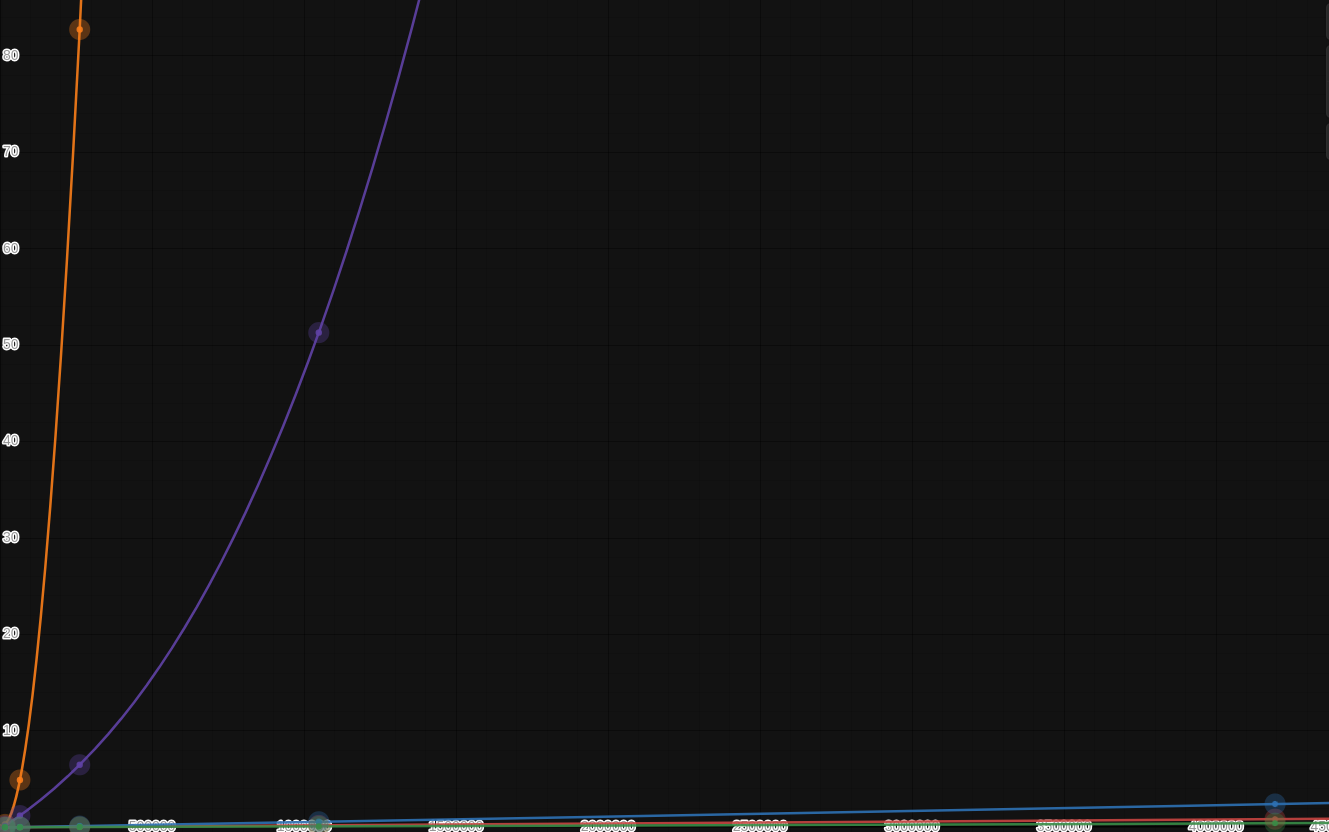
\includegraphics[width=0.90\textwidth]{graph1.png}
    \caption{Графік залежності часу виконання алгоритму від кількості елементів}
\end{figure}
\begin{figure}[H]
    \centering
    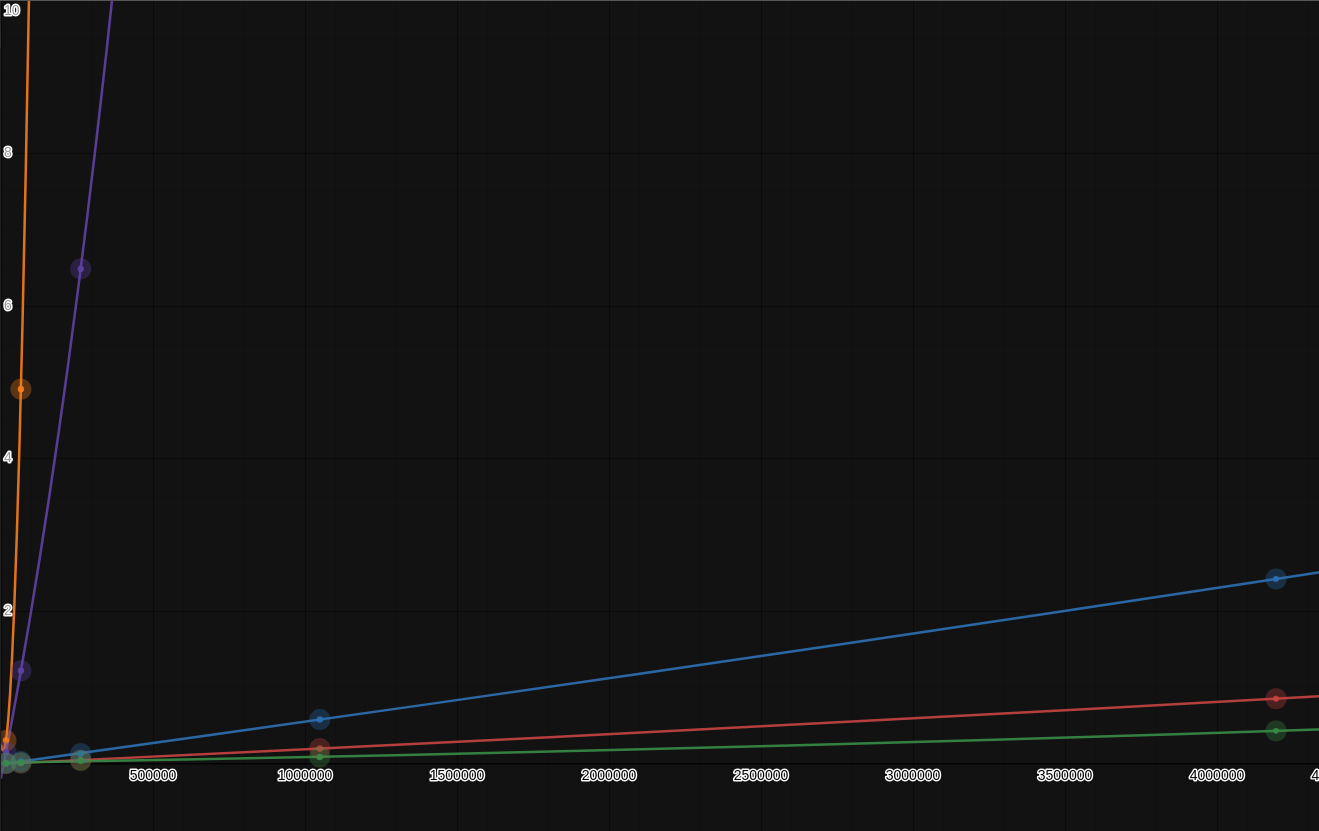
\includegraphics[width=0.90\textwidth]{graph2.png}
    \caption{Оранжевий - Insertion Sort, 
    Фіолетовий - Shell Sort, 
    Синій - Quick Sort, 
    Червоний - Merge Sort,
    Зелений - Counting Sort}
\end{figure}
\begin{figure}[H]
    \centering
    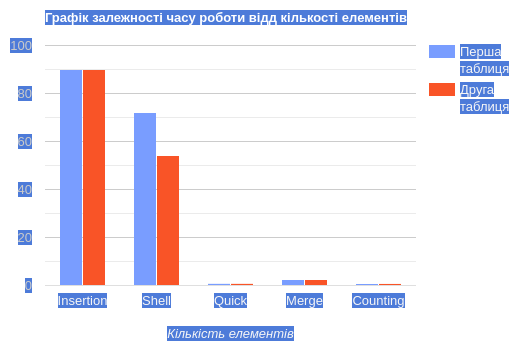
\includegraphics[width=0.90\textwidth]{graph3.png}
\end{figure}

\subsection*{Висновок} 
Сортування - це фундаментальний процес в обробці даних, і для різних випадків використовуються різні алгоритми. Ось короткий висновок про п'ять різних алгоритмів сортування:

Insertion Sort - простий інтуїтивний алгоритм, який добре працює для невеликих списків або вже відсортованих даних. Його складність у найгіршому та середньому випадку - $O(n^2)$, що робить його менш практичним для великих списків.

Shell Sort - вдосконалений варіант сортування вставкою. Він використовує послідовність кроків для поступового зменшення відстаней між елементами, що робить його ефективнішим для великих списків. Складність в середньому випадку залежить від конкретної послідовності і дорівнює $O(n log^2 n)$.

Quick Sort - швидкий та ефективний алгоритм, який використовує стратегію розділення і підкорінчення для сортування. У середньому випадку має складність O(n log n), але в найгіршому - $O(n^2)$. Він широко використовується завдяки швидкості та можливості сортувати великі обсяги даних.

Merge Sort - стабільний та надійний алгоритм сортування, який гарантує складність O(n log n) у всіх випадках. Вимагає додаткової пам'яті для об'єднання, але володіє широкими застосуваннями для великих списків та об'єднання великих наборів даних.

Counting Sort - надзвичайно ефективний алгоритм для сортування цілих чисел у межах обмеженого діапазону. Він має складність O(n + k), де k - діапазон можливих значень. Counting Sort особливо корисний для великих обсягів даних зі значеннями в цьому діапазоні.

Загалом, вибір алгоритму сортування залежить від специфіки задачі, розміру даних та ресурсів, доступних для виконання сортування.
\end{document}
